%
% https://aws.amazon.com/blogs/architecture/building-a-controlled-environment-agriculture-platform/
% https://d2908q01vomqb2.cloudfront.net/fc074d501302eb2b93e2554793fcaf50b3bf7291/2020/12/21/Data-pipeline-Grov-Technologies-1024x374.png
%\documentclass[border=40pt]{standalone}
\documentclass{article}
\usepackage{tikz}
\usepackage{hyperref}
\usepackage{pdflscape}
\usepackage[export]{adjustbox}

%%% This is the aws icons style
\usepackage{../sty/awsicons} 
%% Also needed!!
\graphicspath{{../icons_tex/}}

%% From: https://tex.stackexchange.com/a/847
\hypersetup{
    colorlinks,
    linkcolor={red!50!black},
    citecolor={blue!50!black},
    urlcolor={blue!80!black}
}

\renewcommand{\familydefault}{\sfdefault}

\definecolor{reactColor}{RGB}{102,255,255}

\begin{document}
\section{Example: AWS Architecture blog: \textit{Building a Controlled Environment Agriculture Platform}}
\noindent Example taken from AWS Architecture Blog\footnote{\url{https://aws.amazon.com/blogs/architecture}}, 
\textit{Building a Controlled Environment Agriculture Platform}\footnote{\url{https://aws.amazon.com/blogs/architecture/building-a-controlled-environment-agriculture-platform/}}, by Ashu Joshi, 2020.12.22.
Original diagrm\footnote{\url{https://d2908q01vomqb2.cloudfront.net/fc074d501302eb2b93e2554793fcaf50b3bf7291/2020/12/21/Data-pipeline-Grov-Technologies-1024x374.png}} recreated, using \href{https://ctan.org/pkg/pgf?lang=en}{tikz} and the \href{https://github.com/gnewton/awsArchIcons2LaTeX}{awsicons} package.
\pagenumbering{gobble}
\newpage
\begin{landscape}
\section{Original diagram (PNG image)}
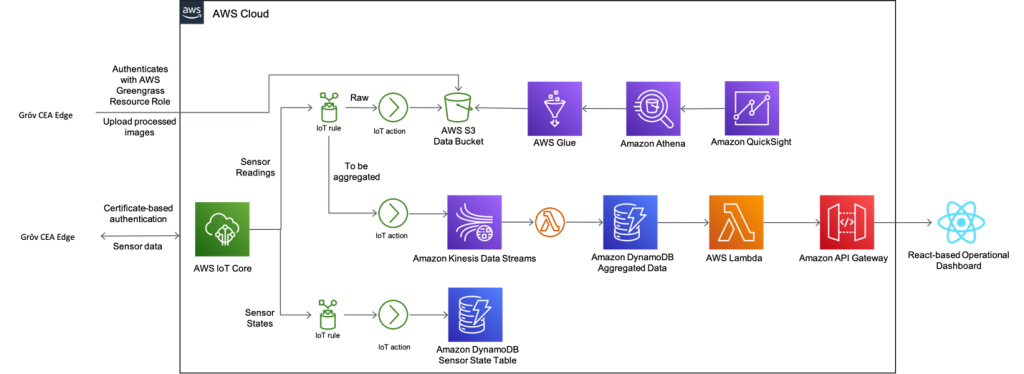
\includegraphics[width=20cm] {Data-pipeline-Grov-Technologies-1024x374.png}

\section{Recreated diagram}
\begin{tikzpicture}[%
    %% AWS has no React symbol
    %% From: https://tex.stackexchange.com/questions/349960/how-to-draw-a-symbol-on-a-tikz-node-that-can-be-reused
    atom/.style = {shape=coordinate,minimum size=#1,
      append after command={%
        \pgfextra{ 
          \foreach \ang in {0,120,240}
          \draw[draw=reactColor,very thick,rotate around={\ang:(0,0)}] (\tikzlastnode.center) ellipse (0.45*#1 and 0.17*#1); 
          \fill[fill=reactColor] (\tikzlastnode.center) circle (0.08*#1);
        }
      }
    }
  ]

  \draw [draw=black,thick] (-1,-3.5) rectangle (13,4.7);


  \node (core) {\AIoTCore{1cm}};
  \node (preCore)[shape=coordinate,left of=core,align=center] {};
  \node (sensorData)[shape=coordinate,left of=preCore,align=center,xshift=-8mm] {};

  \node (botEdge)[black,left of=sensorData,align=center, xshift=-1mm] {\tiny \textbf{Gr\"{o}v CEA Edge}};
  \node (coreLabel)[below of=core,align=center,yshift=3.5mm] {\tiny AWS IoT Core};
  \node (split) [shape=coordinate,right of= core] {};
  \node (topAngle) [shape=coordinate,above of = split,yshift=1.2cm] {};
  \node (botAngle) [shape=coordinate,below of = split,yshift=-1.2cm] {};


  \node (topIotRule)[right of= topAngle]{\RIoTRule{.35cm}};
  \node (topIotRuleLabel)[below of=topIotRule,align=center,yshift=6mm] {\tiny IoT Rule};
  \node (botIotRule)[right of= botAngle]{\RIoTRule{.35cm}};
  \node (botIotRuleLabel)[below of=botIotRule,align=center,yshift=6mm] {\tiny IoT Rule};
  \node (topIotAction)[right of= topIotRule,xshift=5mm]{\RIoTAction{.55cm}};
  \node (topIotActionLabel)[below of= topIotAction,align=center,yshift=6mm]{\tiny IoT Action};
  \node (botIotAction)[right of= botIotRule,xshift=5mm]{\RIoTAction{.55cm}};
  \node (botIotActionLabel)[below of= botIotAction,align=center,yshift=6mm]{\tiny IoT Action};
  \node (midIotAction)[below of= topIotAction,yshift=-1cm]{\RIoTAction{.55cm}};
  \node (midIotActionLabel)[below of= midIotAction,align=center,yshift=6mm]{\tiny IoT Action};
  \node (midAngle) [shape=coordinate,below of = topIotRule,yshift=-1cm] {};

  \node (kinesis) [right of = midIotAction,xshift=.5cm] {\AKinDataStreams{1cm}};
  \node (kinesisLabel)[below of= kinesis,align=center,yshift=2.5mm]{\tiny Amazon Kinesis \\[-2mm] \tiny Data Streams};

  \node (sensorDynamo)[right of= botIotAction,xshift=.5cm]{\ADDB{1cm}};
  \node (sensorDynamoLabel)[below of= sensorDynamo,align=center,yshift=2.5mm]{\tiny Amazon DynamoDB \\[-2mm] \tiny Sensor State Table};

  \node (s3)[right of= topIotAction,xshift=.5cm]{\RSThreeBkt{.55cm}};
  \node (s3Label)[below of= s3,align=center,yshift=4.5mm]{\tiny AWS S3 \\[-2mm] \tiny Data Bucket};

  \node (s3AboveAngle) [shape=coordinate,above of = s3,yshift=-3mm] {};
  \node (images) [shape=coordinate,left of = s3AboveAngle, xshift=-7cm] {};
    \node (topEdge)[black,left of=images,align=center, xshift=-1mm] {\tiny \textbf{Gr\"{o}v CEA Edge}};

  \node (glue)[right of= s3,xshift=1cm]{\AGlue{1cm}};
  \node (glueLabel)[below of= glue,align=center,yshift=3.5mm]{\tiny Amazon Glue};

  \node (athena)[right of= glue,xshift=1cm]{\AAthena{1cm}};
  \node (athenaLabel)[below of= athena,align=center,yshift=3.5mm]{\tiny \textbf{Amazon Athena}};

  \node (quicksight)[right of= athena,xshift=1cm]{\AQuickSight{1cm}};
  \node (quicksightLabel)[below of= quicksight,align=center,yshift=3.5mm]{\tiny Amazon QuickSite};
  
  \node (lambdaFunction)[right of= kinesis,xshift=.5cm]{\RLambdaLambdaFunc{.55cm}};
  \node (aggrDynamo)[right of= lambdaFunction,xshift=.5cm]{\ADDB{1cm}};
  \node (aggrDynamoLabel)[below of= aggrDynamo,align=center,yshift=2.5mm]{\tiny Amazon DynamoDB \\[-2mm] \tiny Aggregated Data};
  \node (lambda)[right of= aggrDynamo,xshift=1cm]{\ALambda{1cm}};
  \node (lambdaLabel)[below of= lambda,align=center,yshift=3.5mm]{\tiny Amazon Lambda};
  
  \node (apiGateway)[right of= lambda, xshift=1cm]{\AAPIGateway{1cm}};
  \node (apiGatewayLabel)[below of= apiGateway,align=center,yshift=3.5mm]{\tiny Amazon API Gateway};

  \node (nearReact) [shape=coordinate,right of= apiGateway, xshift=0.5cm]{};
  \node (react) [draw, atom=9mm, right of= apiGateway, xshift=1.2cm]{};
  \node (reactLabel)[below of= react,align=center,yshift=2.5mm]{\tiny React--based Operational \\[-2mm] \tiny Dashboard};
  
  %%%%%%%%%%%%%%
  \draw[<->,gray] (preCore) -- (sensorData)node[pos=.5,above,align=center, black]{\tiny \textbf{Certificate--based} \\[-2mm] \tiny \textbf{authentication}}  node[pos=.5,below, black,align=center]{\tiny \textbf{Sensor Data}};
  \draw[-,gray]  (images) -- (s3AboveAngle)node[pos=.15,above,align=center, black]{\tiny \textbf{Authenticates} \\[-2mm] \tiny \textbf{with AWS} \\[-2mm] \tiny \textbf{Greengrass} \\[-2mm] \tiny \textbf{Resource Role}} node[pos=.15,below, black,align=center]{\tiny \textbf{Upload processed} \\[-2mm] \tiny \textbf{images}};
  \draw[->,gray]  (s3AboveAngle) -- (s3);
  
  \draw[-,gray]   ([xshift=-1.2mm]core.east) -- (split);
  \draw[-,gray]   (split) -- (topAngle) node[black,yshift=-.9cm,xshift=-1mm,align=center,xshift=-3.5mm]{\tiny \textbf{Sensor} \\[-2mm] \tiny \textbf{Readings}};
  \draw[-,gray]   (split) -- (botAngle) node[black,pos=1,align=center,xshift=-3.5mm]{\tiny \textbf{Sensor} \\[-2mm] \tiny \textbf{States}};

  \draw[->,gray]  (topAngle) -- (topIotRule);
  \draw[->,gray]  (topIotRule) -- (topIotAction) node[black,midway,above,align=center]{\tiny \textbf{Raw}};
  \draw[->,gray]  (botAngle) -- (botIotRule) ;
  \draw[->,gray]  (botIotRule) -- (botIotAction);

  \draw[->,gray]  (botIotAction) -- (sensorDynamo.west);

  \draw[->,gray]  (topIotAction) -- (s3.west);

  \draw[->,gray]  (glue) -- (s3);
  \draw[->,gray]  (athena) -- (glue);
  \draw[->,gray]  (quicksight) -- (athena);

  \draw[-,gray]  (topIotRuleLabel) -- (midAngle)  node[pos=0.5, xshift=-.9mm,right,align=center, black]{\tiny \textbf{To be} \\[-2mm] \tiny \textbf{aggregated}};
  \draw[->,gray]  (midAngle) -- (midIotAction);
  \draw[->,gray]  (midIotAction) -- (kinesis);
  \draw[->,gray]  (kinesis) -- (lambdaFunction);
  \draw[->,gray]  (lambdaFunction) -- (aggrDynamo);
  \draw[->,gray]  (aggrDynamo) -- (lambda);
  \draw[->,gray]  (lambda) -- (apiGateway);

  \draw[->,gray]  (apiGateway) -- (nearReact);

  
    
\end{tikzpicture}
\end{landscape}

\end{document}



